\documentclass{article}

% Language setting
% Replace `english' with e.g. `spanish' to change the document language
\usepackage[english]{babel}

% Set page size and margins
% Replace `letterpaper' with`a4paper' for UK/EU standard size
\usepackage[letterpaper,top=2cm,bottom=2cm,left=3cm,right=3cm,marginparwidth=1.75cm]{geometry}

% Useful packages
\usepackage{amsmath}
\usepackage{graphicx}
\usepackage[colorlinks=true, allcolors=blue]{hyperref}

\title{Esercizio CCS Produttori e Consumatori}
\author{Ruben Castelluccio}

\begin{document}
\maketitle
\section{Introduzione}
L'esercizio consiste nell'Analisi mediante CCS per il problema Produttore - Consumatore.
\\ Si richiede di analizzare 3 diversi modelli di Produttore e Consumatore dove il Buffer è sempre definito a N posizioni:
\begin{itemize}
    \item Primo Setting: 1 Produttore, 1 Consumatore, Buffer a N posizioni;
    \item Secondo Setting: 1 Produttore, 2 Consumatori, Buffer a N posizioni;
    \item Terzo Setting: P Produttori, C Consumatori, Buffer a N posizioni.
\end{itemize}
E' richiesto per ciascun Setting il Modelling Convenience, pertanto discutere se è sempre possibile modellare e la relativa difficoltà costruendo il Derivation Graph per ciascun Setting.
\clearpage
\section{Setting 1}
Nel Primo Setting è richiesto l'utilizzo dei CCS per lo schema Produttore e Consumatore in cui è presente: 1 Produttore, 1 Consumatore e Buffer a N posizioni.
\\Inizialmente il Produttore potrà, solo dopo un azione locale \textit{ploc}, sincronizzanarsi con il Buffer mediante un azione di sincronizzazione \textit{put} andando a modificare il Buffer da E1 (Empty) a F1(Buffer con un inserimento). Successivamente il Consumatore può fare l'azione di sincronizzazione\textit{get} con il Buffer riportandolo in E1 per poi evolevere successivamente con un azione locale \textit{cloc} o in alternativa il Produttore potrà evolvere nuovamente con un azione locale \textit{ploc} per poi inserire una seconda volta nel Buffer.
\\La sincronizzazione avviene mediante azione non osservabile $\tau$ sull'insieme ristretto di azioni \textit{put} e \textit{get} tra il Buffer e il Produttore o il Consumatore.
\\La versione utilizzata del Buffer nel Derivation Graph utilizza un unico Buffer per definire meno stati rispetto alla versione che prevede l'utilizzo della scelta non deterministica (E1 + E1).
In questo Setting si è deciso di limitare al più a 3 inserimenti consecutivi del Produttore nel Buffer, a meno di azioni di sincronizzazione \textit{get} da parte del Consumatore e il Buffer, in quanto viene evidenziata una determinata ciclicità nel Derivation Graph, inoltre ad eccezzione di avere un Buffer vuoto o essere negli stati iniziali si nota che per ogni stato si possono eseguire esattamente 2 azioni che corrispondono a far progredire il Produttore o il Consumatore.
\\Act = \{put,get, ploc, cloc\}
\\Prod = ploc.\underline{put}.Prod
\\Cons = \underline{get}.cloc.Cons
\\E1 = put.F1
\\F1 = put.F2 + get.E1
\\F2 = put.F3 + get.F1
\\F3 = get.F2

\begin{figure}[h] 
\centering
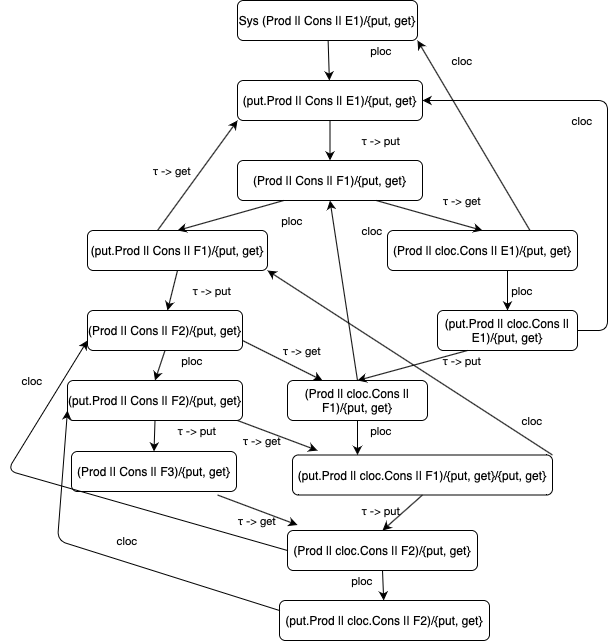
\includegraphics[scale=0.55]{DGSet1.png}
\end{figure}
\subsection{Modelling Convenience}
Nel Setting 1 la principale problematica riscontrata è stata la definizione del Buffer a N posizioni in quanto tale schema prevede la possibilità da parte del Produttore di inserire nel Buffer mediante l'azione \textit{put} senza limiti, per tanto si è deciso di stabilire tale upper bound a 3 inserimenti consecutivi (ovvero senza \textit{get} da parte del Consumatore).
\clearpage
\section{Setting 2}
Nel Secondo Setting è richiesto l'utilizzo dei CCS per lo schema Produttore e Consumatore in cui è presente: 1 Produttore, 2 Consumatori e Buffer a N posizioni.
\\Analogamente a quanto avviene nel Setting 1, all'inizio il Produttore potrà, solo dopo un azione locale \textit{ploc}, sincronizzanarsi con il Buffer mediante un azione di sincronizzazione con il Buffer \textit{put} andando a modificare quest'ultimo da E1 (Empty) a F1(Buffer con un inserimento). Successivamente uno dei due Consumatori potrà fare l'azione di sincronizzazione con il Buffer \textit{get} riportandolo in E1 e dopodichè evolvendo con un azione locale \textit{cloc1} o \textit{cloc2} (a seconda del Consumatore), in alternativa il Produttore potrà fare nuovamente un azione locale per poi inserire una seconda volta nel Buffer. Dopo 2 inserimenti consecutivi nel Buffer da parte del Produttore, i Consumatori potranno prelevare dal Buffer in qualsiasi ordine mediante le azioni di sincronizzazione con il Buffer: \textit{get1} e la \textit{get2}.
\\La sincronizzazione avviene mediante l'azione non osservabile $\tau$ sull'insieme ristretto di azioni \textit{put} e \textit{get1} e \textit{get2} tra il Buffer e il Produttore o i Consumatori.
\\La versione utilizzata del Buffer nel Derivation Graph utilizza un unico Buffer per definire meno stati rispetto alla versione che prevede l'utilizzo della scelta (E1 + E1).
In questo Setting si è deciso di terminare al terzo inserimento del Produttore nel Buffer, a meno di azioni di {get} da parte del Consumatore, in quanto viene evidenziata una determinata ciclicità nel Derivation Graph.
\\Inoltre ad eccezzione di avere un Buffer vuoto o essere negli stati iniziali si nota che per ogni stato si possono eseguire esattamente 3 azioni che corrispondono a far progredire il Produttore, il primo Consumatore o il secondo Consumatore.
\\Act = \{put,get1, get2, ploc, cloc1, cloc2\}
\\Prod = ploc.\underline{put}.Prod
\\Cons1 = \underline{get1}.cloc1.Cons1
\\Cons2 = \underline{get2}.cloc2.Cons2
\\E1 = put.F1
\\F1 = put.F2 + get1.E1 + get2.E1
\\F2 = put.F3 è get1.F1 + get2.F1
\\R = \{put,get1, get2\}
\begin{figure}[h] 
\centering
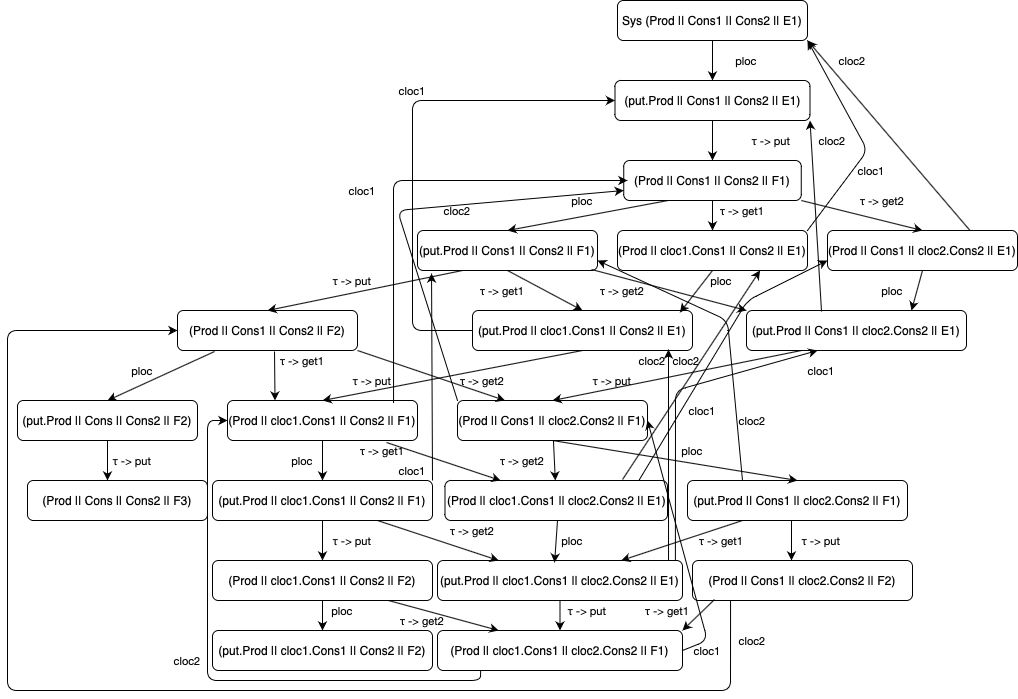
\includegraphics[scale=0.45]{DGSet2.png}
\end{figure}
\subsection{Modelling Convenience}
Nel Setting 2 la principale problematica riscontrata è stata la definizione di un secondo Consumatore e le relative azioni in quanto tale schema prevede la possibilità da parte dei Consumatori di prelevare dal Buffer mediante l'azione \textit{get} con almeno un inserimento avvenuto in precedenza dal Produttore.
\clearpage
\section{Setting 3}
Nel Terzo Setting è richiesto l'utilizzo dei CCS per lo schema Produttore e Consumatore in cui è presente: P Produttore, C Consumatori e Buffer a N posizioni.
\\\\All'inizio i Produttori potranno, solo dopo un azione locale \textit{ploc1} o \textit{ploc2}, sincronizzanarsi con il Buffer mediante un azione di \textit{put1} o \textit{put2} andando a modificare il Buffer da E1 (Empty) a F1(Buffer con un inserimento). Successivamente uno dei due Produttori potrà nuovamente evolvere con un azione locale \textit{ploc1} e \textit{ploc2} per poi inserire una seconda volta nel Buffer o in alternativa i Consumatori potranno fare l'azione di sincronizzazione \textit{get1} o \textit{get2} con il Buffer e dopodichè evolvere con un azione locale \textit{cloc1} o \textit{cloc2} (a seconda del Consumatore). Dopo 2 inserimenti consecutivi nel Buffer da parte di un solo Produttore o di entrambi, i Consumatori potranno prelevare dal Buffer in qualsiasi ordine mediante le azioni di sincronizzazione con il Buffer: \textit{get1} e la \textit{get2}.
\\\\La sincronizzazione avviene mediante azione non osservabile $\tau$ sull'insieme ristretto di azioni \textit{put1} e \textit{put2} e \textit{get1} e \textit{get2} tra il Buffer e i Produttori o i Consumatori.
\\La versione utilizzata del Buffer nel Derivation Graph utilizza un unico Buffer per definire meno stati rispetto alla versione che prevede l'utilizzo della scelta non deterministica(E1 + E1).
In questo Setting si è deciso di terminare al secondo inserimento del Produttore nel Buffer, a meno di azioni di \textit{get} da parte del Consumatore, in quanto viene evidenziata una determinata ciclicità nel Derivation Graph.
\\Inoltre ad eccezzione di avere un Buffer vuoto o essere negli stati iniziali si nota che per ogni stato si possono eseguire esattamente 4 azioni che corrispondono a far progredire il primo Produttore, il secondo Produttore, il primo Consumatore o il secondo Consumatore.
\\\\Act = \{put1, put2, get1, get2, ploc1, ploc2, cloc1, cloc2\}
\\Prod1 = ploc1.\underline{put1}.Prod1
\\Prod2 = ploc2.\underline{put2}.Prod2
\\Cons1 = \underline{get1}.cloc1.Cons1
\\Cons2 = \underline{get2}.cloc2.Cons2
\\E1 = put1.F1 + put2.F1
\\F1 = put1.F2 + put2.F2 + get1.E1 + get2.E1
\\R = \{put1, put2, get1, get2\}
\begin{figure}[h] 
\centering
\fbox{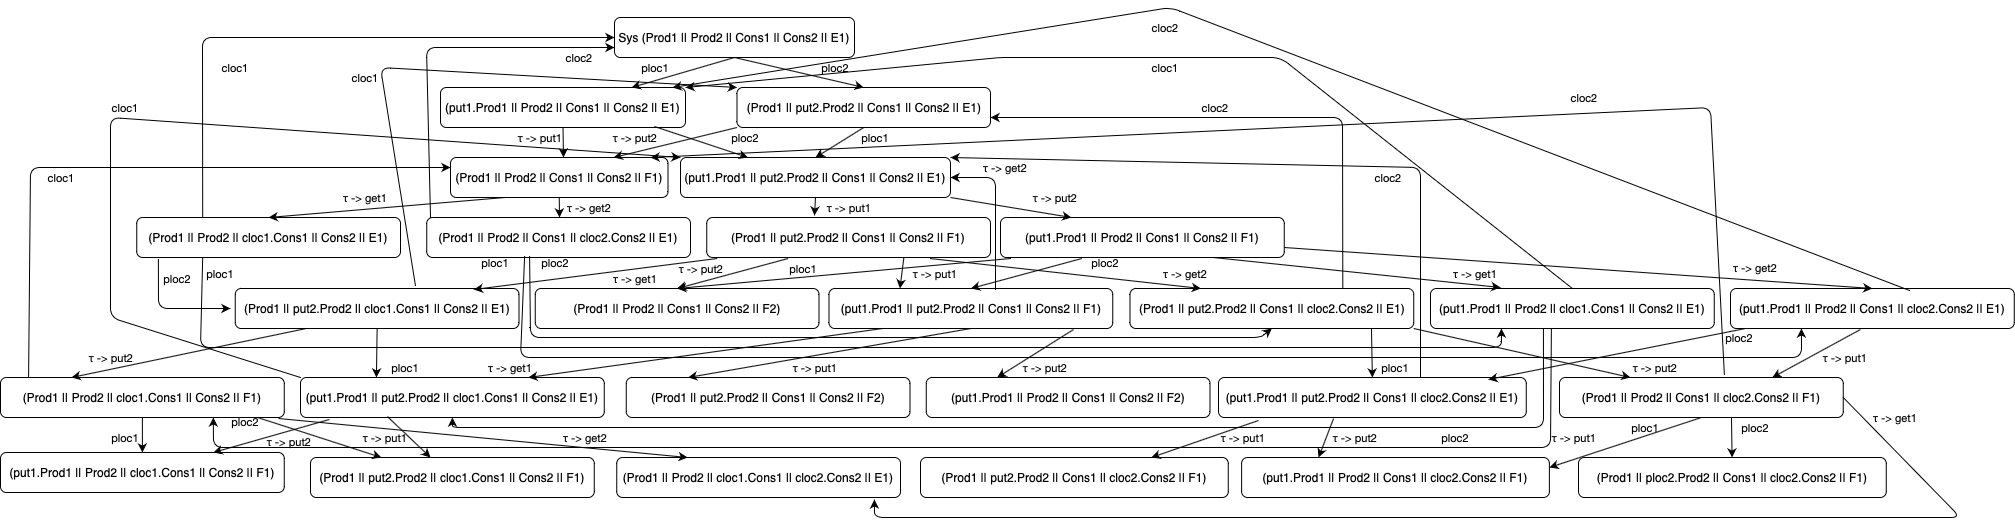
\includegraphics[width=1.15\textwidth, height=2\textheight, keepaspectratio]{DGSet3.png}}
\end{figure}
\subsection{Modelling Convenience}
Nel Setting 3 la principale problematica riscontrata è stata la definizione di un secondo Produttore e le relative azioni in quanto tale schema prevede la possibilità da parte dei Produttori di inserire nel Buffer mediante l'azione di sincronizzazione con il Buffer \textit{put1} e \textit{put2} in qualunque ordine.
\end{document}